\documentclass[../DC2017114Bouma.tex]{subfiles}
\begin{document}
\graphicspath{{03_Contribution/img/}}
\renewcommand{\chaptermark}[1]{\markboth{\thechapter.\ #1}{}}
\renewcommand{\sectionmark}[1]{\markright{#1}{}}

\pagestyle{fancyreport}
\cleartooddpage
\pagestyle{fancyreport}
\chapter{Tracking for Hybrid Systems: Ordered State-Input-Triggered Events}\label{ch:order}
In this chapter a control strategy is presented for trajectories of hybrid systems which, due to the introduction of perturbations, experience ordered state-input-triggered events. Such systems are called \textit{nonlinear state-input triggered hybrid systems} (NSITHS). In this chapter the order of events is always known, but the event-time of each event can vary. The perturbations can cause the state trajectory to jump at a different time than the nominal reference trajectory, resulting in \textit{peaking behavior} of the tracking error \cite{Menini2001,Biemond2013}. First a notion of error \cite{Rijnen2017} is presented, which is used to avoid peaking behavior. After that, similar to the linearization presented in \cite{Rijnen2017}, a first-order approximation of the NSITHS is presented in the form of a \textit{linear time triggered hybrid system} (LTTHS). A proof is given in \cite{Rijnen2017}, which shows that the stability of the LTTHS can be used to asses the local stability of the original NSITHS. Consequentially, conventional stability analysis tools for LTTHS can be used to asses the local stability of te NSITHS. Finally, a short summary of the findings in this chapter is given.

\section{State-input perturbations in trajectories with state-jumps}
\textbf{ADD ASSUMPTIONS 1-6 FROM RIJNEN2017}\\
This section presents \textit{reference-spreading} (RS) for ordered guard activations. First the tracking problem is presented. The perturbations introduced in the state trajectory cause the state trajectory and reference trajectory to have non-coinciding event-times. This mismatch in event-times results in peaking behavior in the tracking error, meaning that two relatively large jumps can be observed. Using reference-spreading this peaking behavior can be avoided, resulting in a tracking error where only one relatively smaller jump is observed.

\subsection{Nonlinear state-input triggered hybrid systems}
As presented in Section~\ref{sec:2hyb}, a mechanical system can be described by the hybrid system with impulsive effects framework. Such a system is given by
\begin{equation}
\begin{array}{ll}
\dot{\xb}(t,i) =\fb_i(\xb(t,i),\ub(t,i),t),& \xb(t,i),\ub(t,i)\notin D_i\\
\xb(t,i) = \gb_i(\xb(t,i-1),\ub(t,i-1),t),& \xb(t,i-1),\ub(t,i-1)\in D_i
\end{array}\label{eq:3hybimp}
\end{equation}
where $\xb(t,i-1),\ub(t,i-1)\in D_i$ triggers the event $\xb(t,i) = \gb_i(\xb(t,i-1),\ub(t,i-1),t)$. The nominal trajectory of such a system is illustrated in Figure~\ref{fig:3perturbedtraj} in orange.
\begin{figure}[h]
\centering
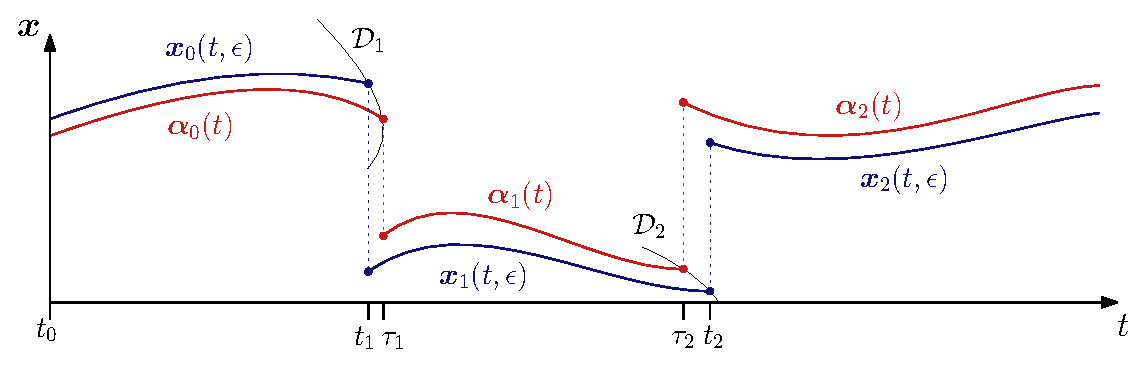
\includegraphics[width=.8\textwidth]{perturbedtraj.eps}\caption{In orange the nominal (unperturbed) and in cyan the perturbed trajectory of a hybrid system with impulsive effects. Due to the perturbation in the cyan trajectory, a mismatch between the perturbed and the nominal event times arises.} \label{fig:3perturbedtraj}
\end{figure}
\textbf{DEFINE PERTURBATIONS} For the nominal trajectory the state and input are known over the entire time-domain, meaning that the event-times are also known. For the perturbed trajectory this is not the case. Due to the uncertainty in the state and input, there is an uncertainty in the event-times as well. This uncertainty can cause a mismatch between the nominal event times $\tau_1$,$\tau_2$ and the perturbed event times $t_1$,$t_2$. Now we take a closer look at the first event, to illustrate the peaking behavior as a result of a jump mismatch. In Figure~\ref{fig:3peakerror} the state evolution $x$ of the first event is depicted besides the tracking error $||x-\alpha$. Here on can clearly see that a peak arises in the tracking error when the jump times do not coincide. At $t_1$ the state trajectory jumps, while the reference trajectory does not. At $\tau_1$ the reference trajectory jumps as well. This means that in $[t_1,\tau_1]$, a post-event state trajectory is compared to a ante-event reference trajectory, resulting in a large peak in the tracking error. This is undesirable, as it will lead to large and unnecessary actuation forces.
\begin{figure}[h]
\centering
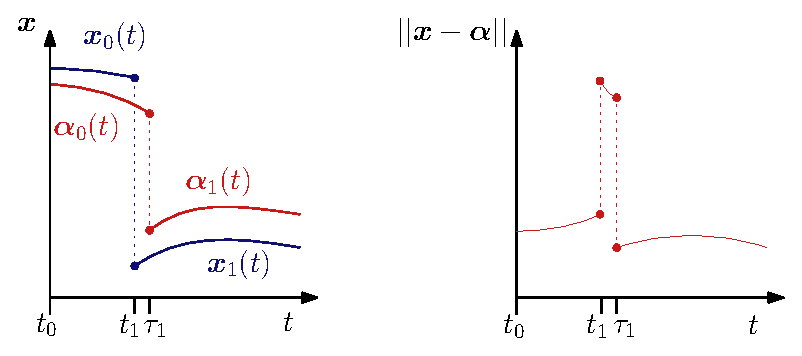
\includegraphics[width=.66\textwidth]{peakerror.eps}\caption{A closer look at the first event of the trajectory in Figure~\ref{fig:3perturbedtraj}. On the left the state-evolution $x$ is depicted and on the right the tracking error $||x-\alpha||$. A clear peak can be noticed in the tracking error as a result from the event-time mismatch.} \label{fig:3peakerror}
\end{figure}

\textbf{Stability definition from Rijnen2017, intuitive explantion of proof in Rijnen2017 that stability of LTTHS -> stability of NSITHS.} In the next section a solution to the peaking behavior is presented.

\subsection{Reference-spreading}
To avoid peaking behavior in the tracking error, in \cite{Saccon2014} a novel notion of error is presented which is named reference spreading in \cite{Rijnen2016}. This control strategy uses reference trajectories which are extended beyond event-times, such that an ante-event state trajectories can always be compared to an ante-event reference trajectory and a post-event state trajectories can always be compared to a post-event reference trajectory. This is illustrated in Figure~\ref{fig:3refspread}, where the reference trajectory segments $\alpha(t,i)$ are all extended resulting in $\overline{\alpha}(t,i)$.
\textbf{DOMAIN DEFINITION}
\begin{figure}[h]
\centering
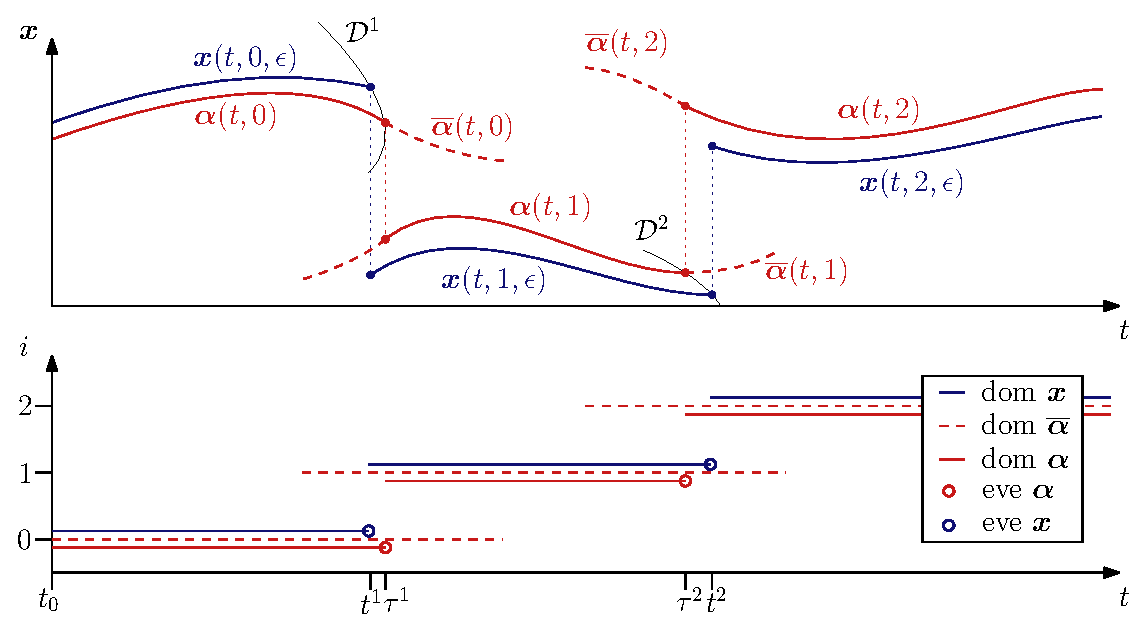
\includegraphics[width=.8\textwidth]{refspreaddom.eps}\caption{An illustration of the nominal reference trajectory (orange) and the perturbed trajectory (cyan), where the nominal reference trajectory is extended such that $\dom x\subseteq\dom \overline{\alpha}$.} \label{fig:3refspread}
\end{figure}

In the lower plot of Figure~\ref{fig:3refspread} the domains of $x$, $\alpha$ and $\overline{\alpha}$ are illustrated for each segment. Note that for every segment, $\dom x(t,i)\subseteq\dom \overline{\alpha}(t,i)$. This means that when the tracking error is defined as $||x-\overline{\alpha}||$, we can keep tracking the error $||x(t,i)-\overline{\alpha}(t,i)||$ until an event is detected. Even if the event-time $t_i>\tau_i$. When an event is detected, the error  $||x(t,i+1)-\overline{\alpha}(t,i+1)||$ can be tracked. Again, because $\dom x(t,i+1)\subseteq\dom \overline{\alpha}(t,i+1)$, this is also possible for the case where $t_i<\tau_i$. Using this notion of error leaves only one jump in the tracking error, even under the presence of event-time mismatches. More importantly, the peak in the tracking error is avoided, an ante-event state trajectory will not be compared to a post-event reference trajectory (and vice versa) anymore. In Figure~\ref{fig:3refspreaderrors} the tracking error with and without reference spreading are compared. Here it is clear that the tracking defined using reference spreading does not have the peak which the normal notion of error does have. It also jumps only once at the perturbed event-time $t_1$.
\begin{figure}[h]
\centering
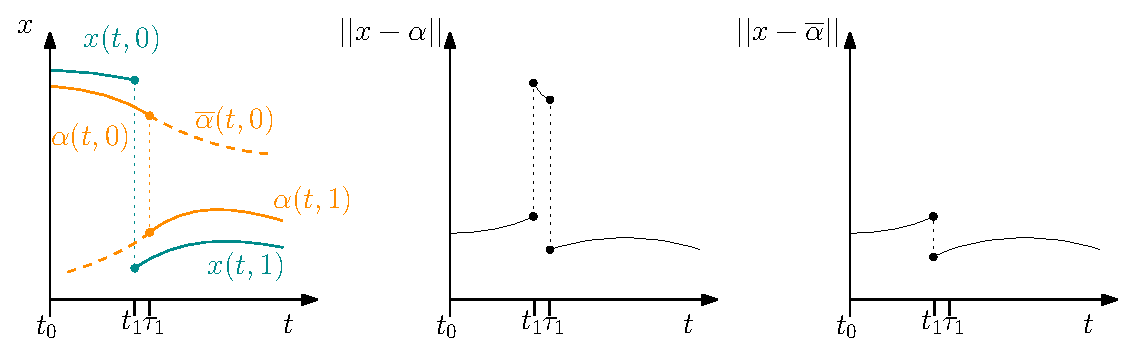
\includegraphics[width=\textwidth]{refspreaderrors.eps}\caption{} \label{fig:3refspreaderrors}
\end{figure}

In the next section the error defined using reference spreading is used to make a first-order approximation of perturbed trajectories with ordered guard-activation.
\section{First-order approximation of trajectories with ordered guard-activations}
Use Rijnen2017 alot
\begin{itemize}
\item LTTHS (Rijnen2017)
\item Jumps at $\tau$ instead of $t$ (also, generally infeasible)
\item First-order accuracy (Rijnen2017)
\item Transversality
\end{itemize}
\section{Stability analysis for linear time-triggered hybrid systems}

\section{Summary}


%% new chapter %%
\cleartooddpage
\chapter{Tracking for Hybrid Systems: Simultaneous State-Input-Triggered Events}\label{ch:simult}
\cite{Rijnen2018}
\section{Simultaneous guard-activation}
\begin{itemize}
\item Simultaneous events and assumptions(same post-event mode,associativity)
\item Event character, mode descriptor, micro counter, historical notation
\item Unidirectional event completion
\end{itemize}
\section{First-order approximation for trajectories with simultaneous guard-activation}
\begin{itemize}
\item Positive homogeneity
\item Positive homogeneous jump gain
\item PHTTHS (Positive homogeneous time-triggered hybrid system)
\end{itemize}

\section{Stability analysis for positively homogeneous time-triggered hybrid systems}

\section{Summary}
\end{document}